% Appendices of the Naming Turn module. Tables 1-4 are generated by figures.py into
% ../outputs/tables/ and re-wrapped (numbers unchanged) by tables/make_tables.py.

\section{Hypothesis ledger}
\label{app:nt-ledger}

Table~\ref{tab:hypotheses} gives every pre-specified hypothesis with its prediction, the pilot value quoted in the locked plan, the final estimate, the final post-audit verdict and the Holm-adjusted $p$ within its direction's family (D1 the naming turn, D2 carriers, D3 LLM wording, D4 peer review). The camera-ready audit's own claims (WP4) are:
\begin{itemize}
\item supported: SB1 (\NAME{} decision-stage association not identified), SB4 (differential findability), V7a (route validation) and G1 (\NAME{} neutrality survives editing);
\item partially supported: SB3 (rare lexical features unauditable), V7b (title stability) and G4 (direction of abstract editing);
\item not supported: SB2 (some feature passes the gate), SB5 (camera-ready retitling excess), G2, G2b and G3 (depletion gates for LLM-title, outsider and abstract markers).
\end{itemize}

% derived from outputs/tables/table1_hypotheses.tex by paper/tables/make_tables.py (numbers unchanged)
{\scriptsize
\begin{longtable}{l p{2.5cm} p{2.2cm} p{3.9cm} p{3.2cm} r}
\caption{Pre-specified hypotheses (locked plan): estimates and final post-audit verdicts (discovery split; all numbers regenerated after the three audits of each direction).}\label{tab:hypotheses}\\
\toprule
ID & Prediction & Pilot (plan) & Estimate (95\% CI) & Final verdict (post-audit) & Holm p \\
\midrule
\endfirsthead
\multicolumn{6}{l}{\textit{Table \ref{tab:hypotheses}, continued}}\\
\toprule
ID & Prediction & Pilot (plan) & Estimate (95\% CI) & Final verdict (post-audit) & Holm p \\
\midrule
\endhead
\bottomrule
\endfoot
\multicolumn{6}{l}{\textit{D1 The naming acceleration: content, composition or tool}} \\
H1a & Slope change at 2024, OR $>$ 1; holds in NA pool; placebo breaks null & OR 1.28/yr (colon titles, not NAME) & OR 1.096 [0.990, 1.214]/yr (year level); paper level 1.098 [1.044, 1.154]; NA pool 1.121 [1.019, 1.232]; sup-LR selects 2023 & Partially supported: the trend accelerated, but a dated 2024 break is not identified (year-level CI includes 1; null without 2026) & 0.071 \\
H1b & Name-masked content share of the 2023$\rightarrow$26 rise in [0.20, 0.50]; none $\geq$ 0.60 & 29\% fixed; 42\% rolling; 45\% unmasked bge & Fixed: R1 0.39 [0.35, 0.43], R3 0.49; rolling: R1 0.57 [0.53, 0.62], R3 0.58 & Not falsified, prediction fails: content share 0.37-0.65 across specifications; 'minority' not established & 0.18 \\
H1c & Unexplained drift u accelerates: mean u(2024--26) - mean u(2019--23) $>$ 0, ratio $\geq$ 1.5 & 1.7 $\rightarrow$ 3.9 pp/yr (ratio 2.3) & u 1.51 $\rightarrow$ 2.87 pp/yr; diff +1.35 pp [0.03, 2.71] (year level); NA pool +1.14 pp & Not established at the year level (positive point estimate; fails Holm; CI includes 0 in NA pool and non-LLM subset) & 0.067 \\
H1d & Composition (team size $\times$ new keys $\times$ LLM topic) explains $\leq$ 30\% (DFL) & 26\% (size $\times$ LLM topic) & DFL 0.29 / 0.32 / 0.26 [0.22, 0.30] (2024/25/26) & Partially supported: met in 2024 and 2026, not in 2025; far from the 0.50 line & 0.008 \\
H1e & Tool bounded: F = 0 rise $\geq$ 85\% of total; $\delta$ $\leq$ 5 pp; tool share at A = 0.39 $<$ 0.25 & colon adjOR 1.24 & F = 0 rise / total 0.98 [0.96, 1.00]; $\delta$ +1.6 pp; tool share 0.07 [0.01, 0.13]; positive control on F\_d1: slot OR 1.29 [0.92, 1.81] & Supported as pre-registered for the abstract fingerprint; not robust as a bound; D3 positive control fails on D1's own fingerprint & 0.002 \\
\addlinespace
\multicolumn{6}{l}{\textit{D2 Who carries the change (declared profile keys)}} \\
H2a & Within-stayer share $\geq$ 0.70 (last position), $\geq$ 0.60 (any position) & last $\approx$ 1.00; any 0.83 & $\rho$\_last 0.995 [0.943, 1.050]; $\rho$\_any 0.816 [0.777, 0.857]; generational null 0.78--0.93 & Not identified: a generational null with the observed co-authorship also meets it & 0.005 \\
H2b & First-position share lower than last by $\geq$ 0.2; entrant first keys above stayers & first 0.58 vs last 1.00 & $\rho$\_first 0.525 [0.414, 0.633]; first - last $-$0.47 [$-$0.60, $-$0.36] & Supported on pre-registered groups; magnitude not robust & 0.005 \\
H2c & Stayer change at zero new co-author keys $\geq$ 0.5 $\times$ population change & 0.60 (rolling) & 0.34 [0.19, 0.48] $\times$ population (6.2 of 18.3 pp) & Not supported (not falsified): newcomer-free teams changed less than predicted & 0.31 \\
H2d & Slope of within-stayer on population change $\approx$ 1; G larger for style than topic & slope 0.97 & slope 0.92 [0.90, 0.95]; G\_style 0.17 [0.13, 0.20] vs G\_topic $-$0.05 [$-$0.07, $-$0.03] & Supported for the style-vs-topic contrast; slope criterion not diagnostic & 0.005 \\
H2e & Pre-LLM (2018$\rightarrow$20, email keys): $\geq$ 50\% of the NAME rise within stayers & -- & $\rho$\_NAME 1.20 [0.71, 1.77]; literal Kitagawa share 0.26 & Inconclusive & 0.12 \\
S2.1 & Retitled resubmissions (destination $\geq$ 2024) do not add NAME on net & 0.000 (se 0.025; 28/28; n = 297) & $\Delta$NAME +0.000 (se 0.025; 28 adds, 28 drops, n = 297); minus topic-adjusted drift $-$4.8 pp & NAME not added on net within retitled projects; lag behind drift not established & expl. \\
S2.2 & Future-tie placebo: past-collaborator exposure no larger than future-collaborator exposure & past .045 vs future .118 & past $-$0.007 vs future +0.067; difference $-$0.075 (se 0.037; MDE 0.10) & Inconclusive: positive control not detected in the primary specification & expl. \\
\addlinespace
\multicolumn{6}{l}{\textit{D3 The machine register}} \\
H3a & Meaning-fixed LLM slots: post OR $\geq$ 2; controls in [0.67, 1.5]; slot - control $>$ 0 & 2.69 [1.80, 4.01]; controls 0.87 & slots 2.18 [1.41, 3.38]; controls 0.87 [0.64, 1.18]; stacked 2.55 [1.53, 4.25] & Supported (pre-registered spec); OR $>$= 2 depends on 'enhancing'; not sharply dated against 2023; addition rather than substitution & $<$0.001 \\
H3b & 2025$\rightarrow$26 within area: R24 falls in $\geq$ 10/16, R26 rises in $\geq$ 12/16 & R24 down 12/16; R26 up 16/16 & R24 down 14/16, R26 up 16/16; R24 relative to neutral synonyms 1.08 [0.86, 1.36] & Thresholds met (descriptive); no register turnover identified & 0.004 \\
H3c & Vintage alignment: OR(F24 $\rightarrow$ R24) $>$ OR(F26 $\rightarrow$ R24), 2025--26 & 1.29 vs 0.83 & 1.11 vs 0.76; ratio 1.46 [1.17, 1.83]; shared-lemma-free 1.32 [1.04, 1.66] with OR(F24) 1.00 & Prediction met; vintage reading not established & 0.001 \\
H3d & Lexical signature: OR(F $\rightarrow$ slot variant) $\geq$ 1.5 $\times$ OR(F $\rightarrow$ NAME) & $\approx$ 2.7 vs $\approx$ 1.24 & OR\_slot 1.42 [1.14, 1.79] vs OR\_NAME (all papers) 1.14 [1.08, 1.21]; ratio 1.24 [0.99, 1.57] (same-paper comparator, collider-conditioned: 1.55) & Partially supported: ratio $>$ 1 marginal against the population comparator; 1.5x not met & 0.030 (pop.) \\
H3e & Exploratory: second-hand diffusion claimed only if U$^{*}$ $>$ 0.8 & $\approx$ 0.55 (2024) & U$^{*}$ 0.65 [0.50, 0.81]; contamination-corrected 0.45 & Unresolved (exploratory): no second-hand-diffusion claim & expl. \\
\addlinespace
\multicolumn{6}{l}{\textit{D4 The gatekeeper (2024--26 pooled)}} \\
H4a & NAME accepted/all in [0.95, 1.10] every year; TOST in [0.90, 1.11]; equal break across pools & 1.01--1.04 (2024--26) & G\_total 1.021 (90\% CI 1.001--1.041; editing-corrected [0.949, 1.031]); pool break ORs (ITS 2018--26) 1.05 / 1.12 / 1.11, p = 0.51 & Supported, robust to camera-ready editing; a small decision-stage premium is not identified & 0.002 \\
H4b & LLM-style and outsider unions depleted (accepted/all $<$ 1); L desk $\times$ exit $<$ 1 & typography 0.79; ALL-CAPS 0.37 & LLM-style 0.975 [0.951, 1.001] (without R24 0.998); desk $\times$ exit 0.981; outsider 0.807 [0.749, 0.870] & Partially supported: L total fails Holm; the L-union depletion is R24-driven and pre-dates 2024 (F24 and style density: new 3-4\% pre-decision depletion); O shortfall not identified as selection & 0.059 \\
H4c & Accepted-only Kobak LLM bound $\leq$ 0.85 $\times$ all-submission bound in each of 2024--26 & 12.8/8.7/3.0 vs 15.8/12.0/5.8 pp & ratios 0.80 / 0.71 / 0.50 (2024 CI [0.66, 0.92]) & Partially supported: direction only; $>$= 15\% not established; falsified under a post hoc pre-ChatGPT baseline & 0.21 \\
H4d & Withdrawn vs rejected: NAME $>$ 0 across papers, $\leq$ 0 within last-position key & +3.6 vs $-$1.4 pp & +4.06 vs $-$0.70 pp; difference 4.77 pp (se 0.75); with topic100 FE cross +0.84 [$-$1.05, 2.74] & Partially supported: contrast holds, but the excess is mostly topic composition & $<$0.001 \\
H4e & Descriptive: published-only atlas within $\pm$10\% for mainstream statistics & -- & mainstream 9/11, outsider 1/4, LLM-style 7/9 within $\pm$10\% & Partially supported (descriptive): prevalences reproduced; 2024 break about half as large (CI $-$0.15 to 1.16) & descr. \\
Gate & A decision-stage gain enters the headline only if its tipping point lies outside the audit CI (Holm across auditable features) & -- & NAME DiD +1.48 pp [$-$0.63, 3.59] vs D$^{*}$ 2.92 pp; 0 of 26 title features pass (18 auditable) & No title-feature acceptance association identified & --- \\
\end{longtable}
\par\noindent \scriptsize Holm p: one-sided, Holm-adjusted within each direction's confirmatory family (D1 uses the year-level tests for H1a and H1c; D1 and D4 p-values test the falsification boundary or an intersection-union of the pre-registered sub-tests; H3d shows the sensitivity family with the population NAME comparator). expl. = exploratory; descr. = descriptive. $\rho$ = stayer-to-population change ratio; G = generational increment; D$^{*}$ = tipping point of the camera-ready net-flip DiD. Discovery-split verdicts are not confirmations; the held-out tests CT1-CT12 are frozen in a hashed bundle (outputs/prereg/). Pilot: value quoted in the locked plan from pilot analyses of the same discovery rows, run before the plan was locked; predictions and thresholds were informed by these pilots. Holm p tests the pre-registered statistic; the verdict also weighs the identification checks added in the audits, so a small Holm p can coexist with `not identified' (e.g.\ H2a).\par
}


\clearpage
\section{Robustness}
\label{app:nt-robust}

Table~\ref{tab:acceleration} reports the \NAME{} acceleration across samples and definitions, and Table~\ref{tab:content} reports the content bracket across representations. Further checks, each documented in the direction outputs:
\begin{itemize}
\item The first-minus-last list-position gap $\rho_{\text{first}}-\rho_{\text{last}}$ excludes 0 in all nine variants: author weighting, the camera-ready-free pool ($-0.426$), excluding 2026, 2026 only, partition-specific stayers, trimming, topic adjustment, dropping email-keyed papers, and a restricted alias collapse ($-0.394$). The most extreme trailing-digit collapse shrinks it to $-0.243$ \ci{-0.344}{-0.133}.
\item The slot result holds with topic100 and bge topic fixed effects (pooled slot OR 2.28 and 2.37). A pilot-like specification (any colon lead, full lexicon) gives 2.80 \ci{1.89}{4.15}.
\item The D4 stage gains are reported with raw pooling, without post-decision withdrawals and excluding 2026.
\item Using the 2021--22 false-positive rate instead of the 2023 one moves the corrected tool share from 7.1\% to 7.4\% \ci{1.4}{13.4}.
\item The \NAME{} decision-stage gain is 1.050 \ci{1.028}{1.072} in D4's stage-gain bootstrap and \ci{1.027}{1.073} in the audit's own bootstrap; the two use different resampling.
\item 2026 sensitivity: see Table~\ref{tab:nt-2026}. Paper-level slope change without 2026: 1.052 \ci{0.964}{1.147}.
\end{itemize}

% derived from outputs/tables/table2_acceleration.tex by paper/tables/make_tables.py (numbers unchanged)
\begin{landscape}
\begin{table}[p]
\centering
\scriptsize
\caption{The NAME acceleration across samples and definitions: segmented-logit ITS and content-unexplained drift.}
\label{tab:acceleration}
\begin{adjustbox}{max width=\linewidth}
\begin{tabular}{l r l l l l l l}
\toprule
Sample / definition & n & NAME 2023$\rightarrow$26 (\%) & Pre-trend OR/yr & Slope change OR/yr & Year-level OR/yr & LPM slope change (pp/yr) & $\Delta$u (pp/yr) \\
\midrule
All submissions (primary) & 43,482 & 20.3 $\rightarrow$ 40.5 & 1.125 & 1.098 [1.044, 1.154] & 1.096 [0.990, 1.214] & +2.97 [+2.13, +3.81] & +1.35 [+0.56, +2.15] \\
Camera-ready-free pool (NA) & 30,322 & 20.1 $\rightarrow$ 40.3 & 1.113 & 1.128 [1.061, 1.199] & 1.121 [1.019, 1.232] & +3.45 [+2.36, +4.55] & +1.14 [+0.14, +2.15] \\
Non-LLM-topic subset & 30,269 & 19.5 $\rightarrow$ 36.0 & 1.120 & 1.116 [1.055, 1.180] & 1.108 [0.986, 1.245] & +3.03 [+2.04, +4.03] & +0.55 [$-$0.38, +1.45] \\
NA pool $\times$ non-LLM & 21,199 & 19.4 $\rightarrow$ 36.4 & 1.112 & 1.145 [1.065, 1.230] & --- & +3.46 [+2.15, +4.77] & --- \\
Accepted pool (2017--26) & 13,048 & 20.6 $\rightarrow$ 40.8 & 1.139 & 1.042 [0.964, 1.127] & --- & +1.96 [+0.61, +3.30] & --- \\
Rejected pool (2017--26) & 19,485 & 18.6 $\rightarrow$ 37.9 & 1.101 & 1.115 [1.031, 1.206] & --- & +3.03 [+1.68, +4.38] & --- \\
Withdrawn pool (2018--26) & 9,954 & 23.6 $\rightarrow$ 43.5 & 1.136 & 1.107 [0.992, 1.235] & --- & +3.20 [+1.34, +5.06] & --- \\
Excluding 2026 & 28,070 & 20.3 $\rightarrow$ --- & 1.126 & 1.052 [0.964, 1.147] & 1.046 [0.807, 1.355] & +2.03 [+0.39, +3.67] & +1.15 [+0.15, +2.19] \\
Without 2019 & 42,234 & 20.3 $\rightarrow$ 40.5 & 1.127 & 1.095 [1.041, 1.151] & --- & +2.93 [+2.09, +3.76] & +1.81 [+0.89, +2.72] \\
NAME strict (one-token lead) & 43,482 & 19.6 $\rightarrow$ 39.4 & 1.129 & 1.098 [1.043, 1.155] & --- & +3.00 [+2.16, +3.84] & +1.14 [+0.34, +1.93] \\
NAME loose ($\leq$ 2-token lead) & 43,482 & 22.2 $\rightarrow$ 42.6 & 1.103 & 1.112 [1.060, 1.166] & --- & +3.03 [+2.18, +3.89] & +1.49 [+0.64, +2.35] \\
Any colon or spaced dash & 43,482 & 32.6 $\rightarrow$ 59.9 & 1.088 & 1.231 [1.176, 1.289] & --- & +5.21 [+4.20, +6.22] & +3.94 [+2.95, +4.94] \\
bge topic100 FE & 43,482 & 20.3 $\rightarrow$ 40.5 & 1.125 & 1.088 [1.035, 1.144] & --- & +2.80 [+1.85, +3.75] & --- \\
No controls, no topic FE & 43,482 & 20.3 $\rightarrow$ 40.5 & 1.153 & 1.188 [1.115, 1.266] & --- & +5.13 [+3.95, +6.31] & --- \\
\bottomrule
\end{tabular}
\end{adjustbox}
\par\smallskip
\parbox{\linewidth}{\scriptsize Segmented logit NAME \textasciitilde{} (t-2023) + post + post$\cdot$(t-2023) + log authors + LLM topic + topic100 FE, 2017-26; slope-change CIs clustered by topic100 (paper level); year-level ORs from a REML random-effects meta-regression on adjusted year effects (t, 6 df). LPM: linear probability analogue. $\Delta$u: mean content-unexplained annual change 2024-26 minus 2019-23 from the rolling name-masked R1 content model (conditional paper bootstrap; the two-stage year-level CI for the primary is in Table~\ref{tab:hypotheses}). --- = not estimated for that sample. Pool rows: accepted and rejected pools 2017-26, withdrawn 2018-26 (the D1 window); D4 fits all three pools on 2018-26 for H4a (Table~\ref{tab:hypotheses}, Figure~\ref{fig:nt-gains}: ACC 1.053 / REJ 1.119 / WD 1.107).}
\end{table}
\end{landscape}

% derived from outputs/tables/table3_content_bracket.tex by paper/tables/make_tables.py (numbers unchanged)
\begin{landscape}
\begin{table}[p]
\centering
\scriptsize
\caption{Content-counterfactual bracket: share of the NAME rise predicted by abstract content, by representation and design.}
\label{tab:content}
\begin{adjustbox}{max width=\linewidth}
\begin{tabular}{l l l l l l l l}
\toprule
Rep. & Representation & Role & Share, fixed window & Share, rolling & Share, placebo (2023) & AUC fixed / rolling & $\Delta$u (pp/yr) \\
\midrule
R1 & Masked abstract TF-IDF (primary) & masked & 0.39 [0.35, 0.43] & 0.57 [0.53, 0.62] & 0.26 [0.16, 0.50] & 0.744 / 0.712 & +1.35 [+0.56, +2.15] \\
R3 & Masked abstract, bge embedding & masked & 0.49 [0.44, 0.54] & 0.58 [0.53, 0.63] & 0.42 [0.27, 0.76] & 0.745 / 0.715 & +1.29 [+0.43, +2.10] \\
R5 & R1 minus rhetorical moves & masked & 0.38 [0.34, 0.43] & 0.56 [0.52, 0.61] & 0.25 [0.15, 0.46] & 0.743 / 0.711 & +1.40 [+0.54, +2.21] \\
R1yfe & R1 + training-year FE & sensitivity & 0.38 [0.34, 0.42] & 0.54 [0.50, 0.59] & 0.21 [0.12, 0.39] & 0.744 / 0.712 & +1.50 [+0.68, +2.28] \\
R1@0.5 & R1 at the pilot's C = 0.5 & sensitivity & 0.22 [0.19, 0.24] & 0.42 [0.39, 0.46] & 0.12 [0.08, 0.21] & 0.746 / 0.715 & +2.08 [+1.30, +2.89] \\
R2 & Author keywords & lower & $-$0.04 [$-$0.06, $-$0.03] & 0.12 [0.10, 0.14] & $-$0.05 [$-$0.16, 0.01] & 0.567 / 0.590 & +3.76 [+2.89, +4.67] \\
R6 & topic100 (MiniLM) + LLM topic & coarse & 0.17 [0.15, 0.20] & 0.33 [0.30, 0.36] & 0.06 [0.01, 0.12] & 0.640 / 0.622 & +2.51 [+1.69, +3.33] \\
R6b & topic100 (bge) + LLM topic & coarse & 0.18 [0.16, 0.20] & 0.33 [0.31, 0.37] & 0.06 [0.03, 0.14] & 0.643 / 0.623 & +2.60 [+1.71, +3.48] \\
R4 & Unmasked abstract, bge & upper (leaky) & 0.55 [0.50, 0.61] & 0.64 [0.60, 0.70] & 0.52 [0.34, 0.96] & 0.759 / 0.734 & +1.01 [+0.21, +1.86] \\
\bottomrule
\end{tabular}
\end{adjustbox}
\par\smallskip
\parbox{\linewidth}{\scriptsize Fixed window: L2 logit trained on 2021-23, intercept recalibrated to 2023, share of the 2023-26 rise. Rolling: one-step-ahead models trained on y-3..y-1, recalibrated to y-1; share of the summed 2024-26 annual changes. Placebo: trained 2018-20, share of the 2020-23 rise. C chosen by 5-fold CV except R1@0.5. AUC: out-of-sample, mean over test years. CIs: conditional paper bootstrap (B = 2000). Claims use the name-masked rows only (R1, R3, R5); R4 leaks names and is an upper bound, R2 and R6 are coarse lower brackets.}
\end{table}
\end{landscape}


\clearpage
\section{Measurement validation}
\label{app:nt-validation}

\paragraph{Detector logic.} A title is compound if it contains a colon (or full-width colon) followed by text, or a spaced hyphen or dash. Its lead is the text before the first such separator. The lead is \NAME{} if it is a single token that is not a function word or a genre label (``Position'', ``Survey'', \dots), a two-token lead whose first token has an inner capital, a digit or at least two capitals (``LLaVA 1.5''), or a phrase ending in a parenthesised acronym. Descriptive two-word leads (``Deep Rewiring'') are phrase colons. The rules and lexicons are in \texttt{src/features.py}, \texttt{src/analyses/features\_v2.py} and \texttt{src/analyses/lexicons.json}.

\begin{table}[h]
\centering
\footnotesize
\caption{Example titles by detector class. All examples are accepted ICLR papers, chosen as the first titles by submission ID within the class and year; slot classes are shown only as templates in the main text, so that no individual paper is implied to be an LLM user.}
\label{tab:nt-examples}
\begin{tabular}{p{3.0cm}p{11.5cm}}
\toprule
Class & Example (year) \\
\midrule
\NAME, mixed case & QANet: Combining Local Convolution with Global Self-Attention for Reading Comprehension (2018) \\
\NAME, ALL-CAPS & GANITE: Estimation of Individualized Treatment Effects using Generative Adversarial Nets (2018) \\
\NAME, word & mixup: Beyond Empirical Risk Minimization (2018); Pyraformer: Low-Complexity Pyramidal Attention for Long-Range Time Series Modeling and Forecasting (2022) \\
\NAME, parenthesised acronym & Blaschke Product Neural Networks (BPNN): A Physics-Infused Neural Network for Phase Retrieval of Meromorphic Functions (2022) \\
\NAME, spaced dash & GenCtrl -- A Formal Controllability Toolkit for Generative Models (2026) \\
Phrase colon (compound, not \NAME) & Deep Rewiring: Training very sparse deep networks (2018) \\
Not compound & Fast Differentiable Matrix Square Root (2022) \\
\bottomrule
\end{tabular}
\end{table}

\begin{itemize}
\item \textbf{V1 (title structure).} We annotated 1,200 stratified main items (six year blocks $\times$ 100 \NAME-positive, 50 phrase-colon and 50 non-compound items) and 200 hard cases (two-token leads, LaTeX, dash compounds, genre and dictionary-word leads). There were two blind passes by LLM annotators (Claude subagents) with different codebooks; model versions were not logged. Cohen's $\kappa$: compound 1.000, question 1.000, lead type 0.949, orthography 0.948, casing 0.969. Of 1,400 items, 58 needed adjudication by the PI's delegate (an LLM agent), and the same agent's spot check of 150 agreed items found 0 clear errors; this check is not independent. The \NAME{} detector (post-stratified) has precision 97.8\% \ci{97.5}{98.3}, recall 97.3\% \ci{96.1}{98.3} and specificity 99.1\% \ci{98.9}{99.3}. Precision varies by 1.2\pp{} across year blocks, and the post-minus-pre difference is $-0.2$\pp{} \ci{-1.3}{0.8}. The misclassification-corrected slope-change OR is 1.090 \ci{1.033}{1.151}, against 1.098 uncorrected.
\item \textbf{V2 (slots).} Three variants were dropped for sense precision below 0.85: exploit/unlocking (0.29), exploit/enabling (0.00) and reveal/decoding (0.39). Swap preservation of the LLM-favoured variants ranges from 0.75 to 0.99; the neutral side of the exploit slot reaches only 0.47--0.70.
\item \textbf{V3 (fingerprints).} False-positive rates in 2021--22 are F24 2.9\%, F26 3.2\%, F\_any 5.9\% and title typography 0.04\%. Spearman correlations with LLM-polish ratings are 0.25 (F\_any), 0.31 (F24) and 0.10 (F26). This is weak convergent validity, and recall is unknown.
\item \textbf{V4 (masking).} The whole-word lead survives R3 masking in 0 of 12,928 \NAME{} abstracts (2018--26) and R1 masking in 22, all project URLs with digit suffixes. Variant spellings survive in 0.36--0.81\% of abstracts. The masked-vs-unmasked AUC gap is $+0.004$ for TF-IDF and $+0.014$ for bge (fixed window).
\item \textbf{V5 (topics).} The LLM-cluster flag agrees with the regex rule at $\kappa=0.86$. MiniLM and bge topic100 partitions agree only moderately (ARI 0.42).
\item \textbf{V6 (keys).} No key-year exceeds 40 papers. Collapsing trailing-digit aliases changes 24.2\% of 2022+ papers' new-key share (mean 0.552 $\rightarrow$ 0.495).
\end{itemize}

\section{Camera-ready audit details}
\label{app:nt-audit}

The audit design has six parts. (1) A stratified random sample of accepted and rejected papers. (2) Pairs: each paper is searched on arXiv and kept if its v1 was posted before that year's decision date. (3) The net-flip DiD: the accepted-minus-rejected difference in net feature flips between v1 and the stored title estimates the camera-ready excess $D$, under the assumption that non-camera-ready edits (arXiv-vs-OpenReview wording, rebuttal edits) occur at the same rate in both arms; we check it by v1 timing. (4) Tipping point: an association is identified only if $D^*$ lies beyond what the audit allows. (5) Auditability: arXiv metadata can carry the feature and at least 10 v1 titles per arm have it. (6) Gate: the editing-corrected 95\% CI must exclude 1, and the identification $p$-value must survive Holm across the 18 auditable title features at one-sided $\alpha=0.025$. The audit also measures differential findability, uses inverse-probability weights for being found, validates the title-search route against a title-free route, and stratifies by when v1 was posted.

\begin{itemize}
\item \textbf{Sample.} The original audit has 616 papers: 75 per year $\times$ decision cell for 2023--26, plus 16 accepted 2022 papers. The enlargement is a fresh stratified sample of 250 per cell for 2023--26 (2,000 records). The frozen sample is the first 2,004 lines of the enlargement cache, with its SHA-256 recorded. Pooled 2023--26 found rates are 86.5\% (accepted) and 53.1\% (rejected), and the usable pre-decision pairs are 803 accepted and 508 rejected.
\item \textbf{Findability.} The odds ratio for being found (accepted) is 5.68 \ci{4.68}{6.89}. \NAME{} does not predict findability (OR 1.00 \ci{0.81}{1.22}). Reweighting by the inverse probability of being found gives a \NAME{} DiD of 1.45\pp{} \ci{-0.81}{3.71}. A title-free search route reproduces the findability gap (0.36 vs 0.36; difference 0.00 \ci{-0.06}{0.06}).
\item \textbf{Retitling.} 23.8\% of accepted and 22.2\% of rejected stored titles differ from v1, a difference of $+1.5$\pp{} \ci{-3.2}{6.1}. Where v1 was posted during review the difference is $-2.7$\pp{} \ci{-7.8}{1.8} (8.7\% vs 11.4\%); where v1 was posted before the deadline it is $+8.6$\pp{} \ci{0.9}{16.1}, so the equal-drift assumption is weakest there.
\item \textbf{Tipping point.} A net camera-ready addition $D$ raises $P(f\mid\text{accepted})=P_3$ by $D$ and $P(f\mid\text{reviewed})=P_2$ by $a_2 D$, where $a_2=0.403$ is the accepted share of the reviewed set. Setting the submission-stage gain $(P_3-D)/(P_2-a_2D)$ to 1 gives $D^*=(P_3-P_2)/(1-a_2)$. For \NAME, $D^*$ is 2.92\pp{} and the audit DiD is $+1.48$\pp{} \ci{-0.63}{3.59} (one-sided identification $p=0.127$).
\item \textbf{Gate.} Of 26 title features, 18 are auditable and none passes the Holm-controlled gate. The smallest Holm-adjusted $p$-values are 0.29 (outsider union without ALL-CAPS), 0.69 (compound) and 0.70 (sentence case). Table~\ref{tab:filter} lists stage gains, audit DiDs and tipping points for every feature.
\item \textbf{Abstracts.} On 2024--26 pairs (628 accepted / 404 rejected), the F24 net-flip DiD is $+0.71$\pp{} \ci{-1.95}{3.36}.
\end{itemize}

% derived from outputs/tables/table4_filter_audit.tex by paper/tables/make_tables.py (numbers unchanged)
\begin{landscape}
\begin{table}[p]
\centering
\scriptsize
\caption{Stage-wise filter gains, ICLR 2024-26, and the camera-ready audit of the decision stage.}
\label{tab:filter}
\begin{adjustbox}{max width=\linewidth}
\begin{tabular}{l r r r r l l l l l}
\toprule
Feature & Share, all (\%) & Desk & Exit & Decision & Total (accepted/all) & Audit & Net-flip DiD (pp) & D$^{*}$ for G\_dec (pp) & Passes gate \\
\midrule
\multicolumn{10}{l}{\textit{Mainstream (M)}} \\
NAME & 35.6 & 0.998 & 0.974 & 1.050 & 1.021 [0.997, 1.044] & yes & +1.5 [$-$0.6, +3.6] & +2.92 & no \\
Compound (any colon) & 53.3 & 0.998 & 0.983 & 1.037 & 1.018 [1.002, 1.034] & yes & +0.7 [$-$1.8, +3.2] & +3.24 & no \\
Phrase colon & 17.7 & 0.999 & 1.002 & 1.011 & 1.012 [0.974, 1.051] & yes & $-$0.7 [$-$2.8, +1.3] & +0.32 & no \\
Mixed-case name & 23.2 & 1.000 & 0.975 & 1.087 & 1.059 [1.029, 1.092] & yes & +1.6 [$-$0.4, +3.7] & +3.29 & no \\
Title Case & 92.9 & 1.000 & 1.001 & 1.017 & 1.018 [1.013, 1.022] & yes & +1.6 [$-$0.6, +3.9] & +2.59 & no \\
\addlinespace
\multicolumn{10}{l}{\textit{Outsider (O)}} \\
ALL-CAPS title & 1.3 & 0.989 & 0.839 & 0.435 & 0.361 [0.260, 0.470] & no (channel) & --- (channel) & --- (channel) & no \\
Sentence case & 4.0 & 1.000 & 1.043 & 0.868 & 0.905 [0.824, 0.985] & yes & +0.8 [$-$1.1, +2.7] & $-$0.94 & no \\
Question opener & 1.8 & 0.974 & 1.013 & 0.911 & 0.899 [0.775, 1.025] & yes & $-$0.1 [$-$1.1, +0.8] & $-$0.26 & no \\
Outsider union & 6.9 & 0.991 & 1.003 & 0.812 & 0.807 [0.749, 0.870] & no (channel) & --- (channel) & --- (channel) & no \\
\addlinespace
\multicolumn{10}{l}{\textit{LLM-style (L)}} \\
LLM typography (title) & 0.7 & 0.981 & 0.979 & 0.975 & 0.936 [0.730, 1.149] & no (channel) & --- (channel) & --- (channel) & no \\
R24 words (title) & 5.3 & 1.000 & 0.901 & 0.896 & 0.807 [0.740, 0.874] & yes & $-$0.2 [$-$1.2, +0.7] & $-$0.83 & no \\
R26 words (title) & 3.6 & 1.004 & 0.965 & 1.093 & 1.060 [0.967, 1.157] & no (count) & $-$0.1 [$-$1.1, +1.0] & +0.54 & no \\
F24 words (abstract) & 12.9 & 1.004 & 0.970 & 0.989 & 0.963 [0.919, 1.011] & yes & +0.7 [$-$1.9, +3.4] & $-$0.23 & no \\
F26 (abstract) & 10.5 & 0.986 & 1.035 & 1.006 & 1.027 [0.978, 1.080] & --- & --- & --- & --- \\
Em dash (abstract) & 6.4 & 0.988 & 1.009 & 0.982 & 0.979 [0.915, 1.049] & no (channel) & --- (channel) & --- (channel) & no \\
Style density (abstract) & 3.26 (mean) & 0.997 & 0.975 & 0.993 & 0.965 [0.955, 0.975] & --- & --- & --- & --- \\
LLM-style union & 33.0 & 0.996 & 0.985 & 0.994 & 0.975 [0.951, 1.001] & --- & --- & --- & --- \\
\bottomrule
\end{tabular}
\end{adjustbox}
\par\smallskip
\parbox{\linewidth}{\scriptsize Gains are P(feature $|$ passed stage)/P(feature $|$ entered stage), year-standardised over 2024-26; total = accepted/all; 95\% CIs from a paper bootstrap stratified by year (B = 2000). Style density is a mean (words per abstract), its gains are ratios of means. Audit: pre-decision arXiv v1 vs stored title (abstract for F24 and em dash), accepted minus rejected net flips (pseudo-flip Wald 95\% CI); a feature is auditable with $>$= 10 v1-present titles in both arms and if arXiv metadata can carry it (arXiv titles are never ALL-CAPS or U+2011/U+2013-typographic; arXiv abstracts carry TeX dashes). Complete audit: original + enlargement, 2023-26 pre-decision pairs (abstracts: 2024-26 pairs). D$^{*}$ for G\_dec: net-flip DiD that would bring the decision gain to 1 (for F24 the G\_total tipping point, used by WP4's gate G3, prereg CT10 and Figure~\ref{fig:nt-bias}b, is $-$0.67 pp). Passes gate: auditable, editing-corrected 95\% CI excludes 1 and the identification p survives Holm across the 18 auditable title features at one-sided 0.025 (F24, em dash: WP4's abstract gate rule). --- (channel): arXiv metadata cannot carry the feature, so the audit's 'net flip' would only restate the stored prevalence; no DiD or D$^{*}$ is reported (WP4 audits the auditable sub-unions R24 or R26 and the O-union without ALL-CAPS in gates G2 and G2b). no (count): fewer than 10 v1-present titles in an arm. --- = not shown: the style density (a mean), the LLM-style union (it contains channel-unauditable parts) and F26 (its abstract words are in WP4's abstract audit, outputs/snapshot/abstract\_audit.csv).}
\end{table}
\end{landscape}


\begin{figure*}[t]
\centering
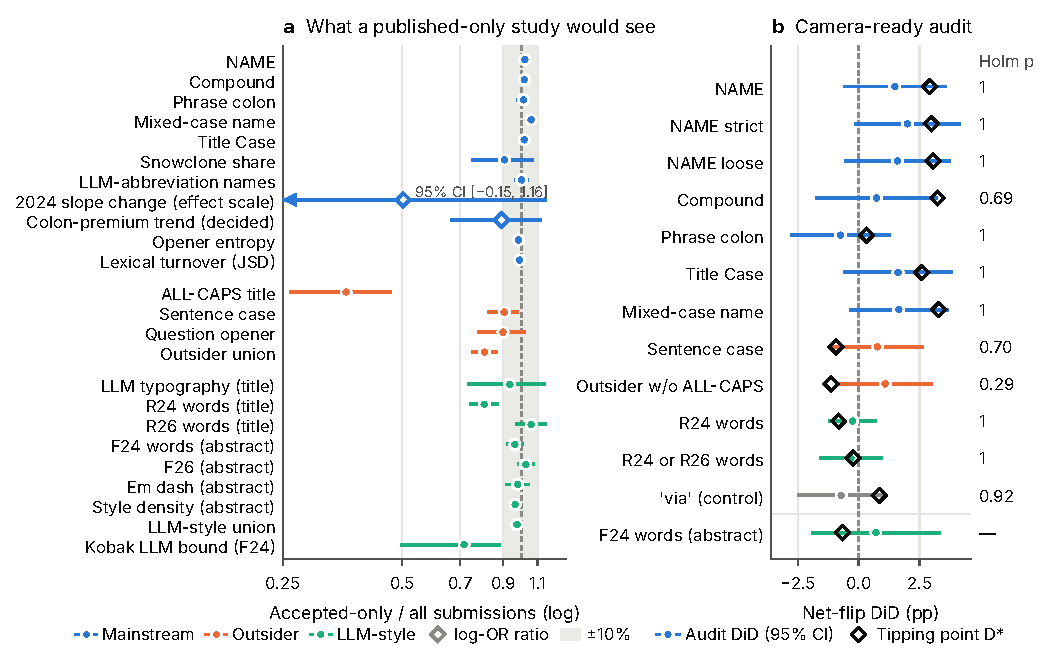
\includegraphics[width=0.95\textwidth]{fig6_published_bias.pdf}
\caption{\textbf{Published-only bias and the camera-ready audit} (2024--26). (a) Accepted-only/all-submission ratios for 24 fashion statistics (95\% CIs; for prevalences the stage-gain bootstrap; dashed: random-selection null bands for entropy and JSD; hollow diamonds: OR statistics compared on the log-OR scale; grey band $\pm 10\%$). The 2024 slope-change row is truncated on the log axis; its CI is \ci{-0.15}{1.16}. (b) Complete arXiv audit (1,311 pre-decision pairs, 2023--26): accepted-minus-rejected net-flip DiD (pseudo-flip 95\% CI) against the tipping point $D^*$, with Holm-adjusted identification $p$ across the 18 auditable title features. Reading rule: an acceptance association is identified only if the whole DiD CI lies short of $D^*$ and the Holm $p$ is below 0.025; no feature meets it. ALL-CAPS titles, title typography and the abstract em dash cannot be audited through arXiv.}
\label{fig:nt-bias}
\end{figure*}

\section{Further results}
\label{app:nt-more}

\begin{figure}[t]
\centering
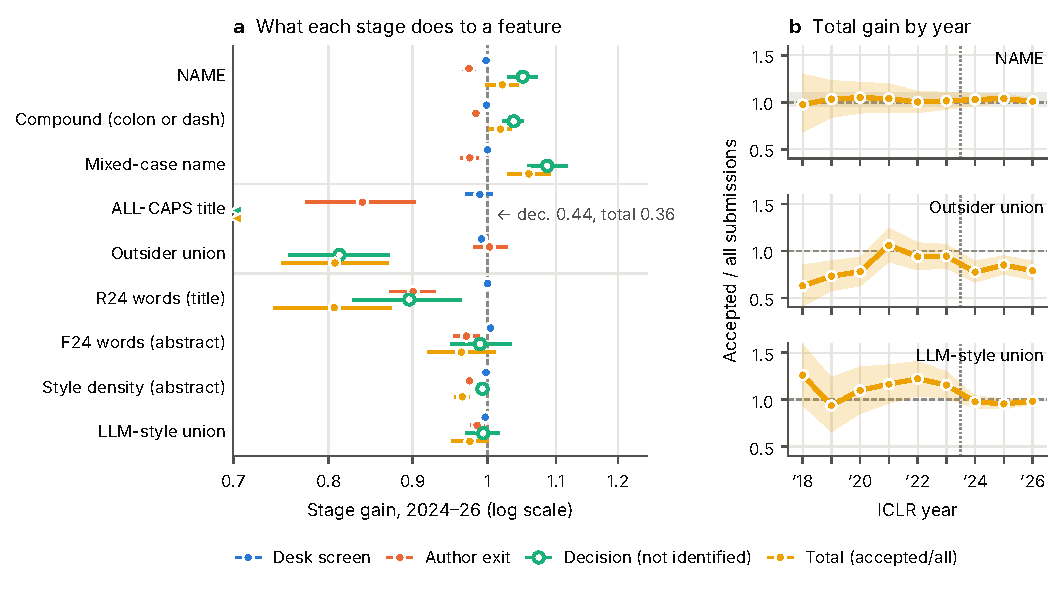
\includegraphics[width=0.92\textwidth]{fig5_stage_gains.pdf}
\caption{\textbf{Stage gains} $P(f\mid\text{passed stage})/P(f\mid\text{entered stage})$, ICLR 2024--26 (year-standardised; paper bootstrap, $B=2000$, 95\% CIs). (a) Desk screen, author exit, decision and total (accepted/all) gains for mainstream, outsider and LLM-style markers; compound $=$ colon or spaced dash. Hollow markers show the decision stage, which is not identified against camera-ready edits. (b) Accepted/all ratio by year; grey band: the pre-specified \ci{0.95}{1.10} band for \NAME. The LLM-style union was enriched among accepted papers in 2018--23 and is not after 2023.}
\label{fig:nt-gains}
\end{figure}

\paragraph{Word families.}
Between 2025 and 2026, 2024 LLM title words fell from 63.1 to 47.8 per 1,000 titles and 2026 LLM title words rose from 23.3 to 46.4 (Figure~\ref{fig:nt-register}b). Their neutral synonyms fell alike (relative RR 1.08 \ci{0.86}{1.36}), and the 2026 family was chosen after a pilot saw it rise, so this is a shift in word families, not an identified register turnover; a title--abstract ``vintage alignment'' contrast (1.46 \ci{1.17}{1.83}) is carried by 2026-fingerprinted papers avoiding 2024 words (Appendix~\ref{app:nt-failures}).

A title--abstract ``vintage alignment'' contrast meets its pre-specified threshold (1.46 \ci{1.17}{1.83}) but, without shared lemmas, the F24 association is OR 1.00, so the contrast is carried by 2026-fingerprinted papers avoiding 2024 words.

\paragraph{Kobak-style bounds.}
Abstracts are our published-only bias case for LLM-use estimates. The all-submission excess-vocabulary bounds are 16.0, 12.2 and 6.0\pp{} (2024--26) and the accepted-only bounds 12.8, 8.7 and 3.0\pp, ratios 0.80 \ci{0.66}{0.92}, 0.71 \ci{0.50}{0.89} and 0.50 \ci{-0.08}{0.93}. The direction holds each year, but the pre-specified $\geq 15\%$ understatement is not established in any year, and under a post hoc pre-ChatGPT baseline the ratios are 0.90, 0.90 and 0.995. Bounds built on a fixed vocabulary decay as model vocabulary changes \citep{geng2025coevolution}: F24 prevalence falls from 19.2\% (2024) to 9.1\% (2026) while F26 rises from 2.5\% to 18.6\%, so the yearly fall of the bounds is not a fall in LLM use.

\paragraph{Withdrawals.}
Among rejected or withdrawn 2024--26 papers, \NAME{} papers are 4.06\pp{} more likely to be withdrawn (cross-section); with topic100 fixed effects the excess is $+0.84$\pp{} \ci{-1.05}{2.74}, so it is mostly topic composition.

\section{What did not hold: full list}
\label{app:nt-failures}

\begin{enumerate}
\item \textbf{No dated 2024 break (H1a, partially supported).} The pilot's slope-change OR of 1.28 per year referred to colon titles, not \NAME. For \NAME{} the estimate is 1.098 at the paper level and 1.096 \ci{0.990}{1.214} at the year level. The pre-specified scan picks 2023, and without 2026 the slope change is null.
\item \textbf{Content is not a minority (H1b).} We predicted 20--50\%; the estimate ranges from 0.37 to 0.65 across specifications. An early ``falsified'' verdict came from a calibration bug, which a review found and we fixed.
\item \textbf{Unexplained drift did not demonstrably accelerate (H1c).} The pre-specified paper bootstrap supported it. Once year shocks are allowed for, it fails Holm (0.067), and its year-level CI includes 0 in the camera-ready-free pool ($+1.14$\pp{} \ci{-0.10}{2.39}) and in the non-LLM subset ($+0.55$\pp{} \ci{-0.90}{1.99}).
\item \textbf{Composition $\leq 30\%$ fails in 2025 (H1d; 0.32).}
\item \textbf{The tool share is not a bound (H1e).} The pre-specified criteria hold for the abstract fingerprint, but the estimate is model-conditional (7\% at the plan's adoption rate, 16--33\% with other markers), and the fingerprint fails a positive control.
\item \textbf{Communal change is not identified (H2a).} Newcomer-free teams changed less than predicted (H2c, $0.34\times$). The pre-LLM test is inconclusive (H2e). A tie-contagion placebo is inconclusive because its positive control is not detected (S2.2).
\item \textbf{No register turnover or vintage alignment (H3b, H3c).} The descriptive thresholds are met, but the neutral-synonym benchmark and the shared-lemma-free contrast (OR for F24 1.00) remove the interpretation.
\item \textbf{The lexical-over-structural ratio is short of $1.5\times$ (H3d)}, and second-hand diffusion is unresolved (H3e).
\item \textbf{Review does not deplete LLM markers as predicted (H4b, partially supported)}, and a $\geq 15\%$ published-only understatement is not established (H4c). The corresponding held-out test (CT10) would now fail its audit gate.
\item \textbf{Claims withdrawn after review.} A camera-ready retitling excess among accepted papers (now $+1.5$\pp{} \ci{-3.2}{6.1}); abstract ``LLM-assisted polishing'' ($+0.71$\pp{} \ci{-1.95}{3.36}); and acceptance associations of compound titles and of outsider casing without ALL-CAPS, which pass only the uncorrected gate (sentence case passed it only at interim audit sizes; all Holm $p \geq 0.29$).
\end{enumerate}

\clearpage
\section{Frozen confirmatory tests}
\label{app:nt-prereg}

Twelve tests are frozen for the held-out split, which has not been requested or seen. The bundle hash is recorded internally and will be deposited publicly before the held-out data are requested. The bundle is revision 3, hash \texttt{6853685bf21a08cdb40227d7fe5d94285c3ec023a9354ab3971faec75051ecd9}. It supersedes revision 2 (\texttt{853827a9\dots}) and revision 1 (\texttt{f69fdb46\dots}). Both revisions were made before any held-out data were requested. Revision 2 re-froze the gate audit on the complete audit and adopted the Holm gate. Revision 3 added reading notes and changed two code paths that no test uses, and every dry-run statistic was unchanged. The primary family CT1--CT6 uses Holm and the secondary family CT7--CT12 uses BH. Table~\ref{tab:nt-ct} gives the discovery dry run. Its ``as if'' verdicts are not confirmations.

\begin{table}[h]
\centering
\footnotesize
\caption{Discovery dry run of the frozen confirmatory tests (revision 3). Source: \texttt{outputs/prereg/dryrun.json}, \texttt{outputs/SUMMARY.md} \S3.}
\label{tab:nt-ct}
\setlength{\tabcolsep}{4pt}
\begin{tabular}{p{4.0cm} p{3.3cm} p{2.9cm} p{4.3cm}}
\toprule
Test & Estimate [95\% CI] & As-if verdict & Reading note \\
\midrule
CT1 D1 break (H1a) & 1.098 \ci{1.044}{1.154} & not confirmed (below minimal effect 1.10) & paper-level SEs; report with the year-level test \\
CT2 drift acceleration (H1c) & $+1.353$ \ci{0.020}{2.701} & not confirmed (CI rule) & within-year resampling cannot establish year-level acceleration \\
CT3 communal change, last position (H2a) & 0.995 \ci{0.943}{1.050} & confirmed & confirms the statistic, not communal change \\
CT4 slot break (H3a) & 2.551 \ci{1.530}{4.255} & confirmed & leans on via/using and \emph{enhancing} \\
CT5 \NAME{} neutral filter (H4a) & 1.021 \ci{1.001}{1.041} (90\%) & confirmed (gate passes) & -- \\
CT6 LLM-marker depletion (H4b) & 0.975 \ci{0.951}{1.001} & not confirmed (gate) & mostly re-detects the pre-2024 R24 depletion \\
CT7 vintage alignment (H3c) & 1.461 \ci{1.168}{1.828} & confirmed & not a vintage test on its own \\
CT8 register shift (H3b) & RR$_{\text{R24}}$ 0.744; RR$_{\text{R26}}$ 1.944 & confirmed & a shift in word families, not turnover \\
CT9 tool bound (H1e(i)) & 0.982 \ci{0.961}{1.004} & confirmed & little power; positive control fails \\
CT10 published-only understatement (H4c) & 0.717 \ci{0.495}{0.888} & not confirmed (gate) & passed only under the revision-1 uncorrected rule \\
CT11 pool invariance (H4a(iii)) & ACC$-$REJ $-0.061$ (90\% \ci{-0.148}{0.027}) & not confirmed & no pair equivalent within $\pm 0.1$ \\
CT12 role gradient (H2b) & $-0.470$ \ci{-0.602}{-0.359} & confirmed & mixes cohort and tenure; not a role effect \\
\bottomrule
\end{tabular}
\end{table}

\section{Reproducibility}
\label{app:nt-repro}

\begin{itemize}
\item \textbf{Code and outputs.} Code is in \texttt{src/analyses/}; run order, runtimes and dependencies are in the study \texttt{README.md}. Each direction's report (\texttt{outputs/d*/RESULTS.md}, \texttt{outputs/snapshot/RESULTS.md}, \texttt{outputs/validation/VALIDATION.md}) ends with an audit response, fix logs are in \texttt{outputs/audit/*/fix\_log.md}, and the consolidated ledger is \texttt{outputs/SUMMARY.\{md,json\}}.
\item \textbf{Figures and tables.} These come from \texttt{python -m analyses.figures}, with captions in \texttt{outputs/figures/manifest.json}.
\item \textbf{Environment.} Python 3.13, CPU only, \texttt{OMP\_NUM\_THREADS=2}, fixed bootstrap seeds. A full re-run takes about 10--12\,h, most of it background embedding and the arXiv enlargement.
\item \textbf{Integrity.} The pre-registration bundle (\texttt{outputs/prereg/bundle.sha256}, 73 files) hashes code, frozen parameters and reference inputs, and \texttt{prereg\_confirm verify} reports no mismatches. The checker scripts pass: D1 153 checks with 3 documented misses, D2 206/0, D3 167/0, D4 108/0, WP4 OK, and the pipeline check has 0 mismatches.
\item \textbf{arXiv caches.} The caches (\texttt{cache/arxiv\_audit*.jsonl}) are gitignored and cannot be reproduced byte for byte by re-querying arXiv. They must be archived separately to regenerate the audit, the slot-word audit and the published-only atlas. Because they link sampled submissions, including rejected ones, to named arXiv records, they are shared only under access control.
\item \textbf{Paper figures.} Figures 1--6 are re-rendered from the same output files by \texttt{paper/figures/make\_paper\_figures.py}, which imports the analysis figure module without changing it and applies the label, colour and panel revisions of review round 1.
\end{itemize}
